
%% bare_conf.tex
%% V1.3
%% 2007/01/11
%% by Michael Shell
%% See:
%% http://www.michaelshell.org/
%% for current contact information.
%%
%% This is a skeleton file demonstrating the use of IEEEtran.cls
%% (requires IEEEtran.cls version 1.7 or later) with an IEEE conference paper.
%%
%% Support sites:
%% http://www.michaelshell.org/tex/ieeetran/
%% http://www.ctan.org/tex-archive/macros/latex/contrib/IEEEtran/
%% and
%% http://www.ieee.org/

%%*************************************************************************
%% Legal Notice:
%% This code is offered as-is without any warranty either expressed or
%% implied; without even the implied warranty of MERCHANTABILITY or
%% FITNESS FOR A PARTICULAR PURPOSE! 
%% User assumes all risk.
%% In no event shall IEEE or any contributor to this code be liable for
%% any damages or losses, including, but not limited to, incidental,
%% consequential, or any other damages, resulting from the use or misuse
%% of any information contained here.
%%
%% All comments are the opinions of their respective authors and are not
%% necessarily endorsed by the IEEE.
%%
%% This work is distributed under the LaTeX Project Public License (LPPL)
%% ( http://www.latex-project.org/ ) version 1.3, and may be freely used,
%% distributed and modified. A copy of the LPPL, version 1.3, is included
%% in the base LaTeX documentation of all distributions of LaTeX released
%% 2003/12/01 or later.
%% Retain all contribution notices and credits.
%% ** Modified files should be clearly indicated as such, including  **
%% ** renaming them and changing author support contact information. **
%%
%% File list of work: IEEEtran.cls, IEEEtran_HOWTO.pdf, bare_adv.tex,
%%                    bare_conf.tex, bare_jrnl.tex, bare_jrnl_compsoc.tex
%%*************************************************************************

% *** Authors should verify (and, if needed, correct) their LaTeX system  ***
% *** with the testflow diagnostic prior to trusting their LaTeX platform ***
% *** with production work. IEEE's font choices can trigger bugs that do  ***
% *** not appear when using other class files.                            ***
% The testflow support page is at:
% http://www.michaelshell.org/tex/testflow/



% Note that the a4paper option is mainly intended so that authors in
% countries using A4 can easily print to A4 and see how their papers will
% look in print - the typesetting of the document will not typically be
% affected with changes in paper size (but the bottom and side margins will).
% Use the testflow package mentioned above to verify correct handling of
% both paper sizes by the user's LaTeX system.
%
% Also note that the "draftcls" or "draftclsnofoot", not "draft", option
% should be used if it is desired that the figures are to be displayed in
% draft mode.
%
\documentclass[conference]{IEEEtran}
% Add the compsoc option for Computer Society conferences.
%
% If IEEEtran.cls has not been installed into the LaTeX system files,
% manually specify the path to it like:
% \documentclass[conference]{../sty/IEEEtran}


\usepackage{times}
\usepackage{epsfig}
\usepackage{graphicx}
\usepackage{amsmath}
\usepackage{amssymb}
\usepackage{subfigure}
\usepackage{caption}
\usepackage{multirow}

%\usepackage{algorithmic}
\usepackage{algorithm}
\usepackage{algpseudocode}
\usepackage{booktabs}
\usepackage{mathtools}
\usepackage{braket}
\usepackage{enumerate}
\usepackage{amsthm}
%------------------------------------------------------------
\DeclareMathOperator*{\argmin}{arg\,min}
\DeclareMathOperator*{\argmax}{arg\,max}
%\numberwithin{equation}{section}
\newtheorem{defi}{Definition}
\newtheorem{theorem}{Theorem}
\newtheorem{lemma}[theorem]{Lemma}

\def\eg{\emph{e.g}.} \def\Eg{\emph{E.g}.}
\def\ie{\emph{i.e}.} \def\Ie{\emph{I.e}.}
\def\cf{\emph{c.f}.} \def\Cf{\emph{C.f}.}
\def\etc{\emph{etc}.} \def\vs{\emph{vs}.}
\def\wrt{w.r.t.} \def\dof{d.o.f.}
\def\etal{\emph{et al}. }
%------------------------------------------------------------

\newcommand{\my}{\mathbf{y}}
%\newcommand{\mnu}{\mathbf{b}}
\newcommand{\mx}{\mathbf{x}}
\newcommand{\ms}{\mathbf{s}}
\newcommand{\mM}{\mathcal{M}}
\newcommand{\mT}{\mathcal{T}}
\newcommand{\mth}{\mathbf{\boldsymbol \theta}}
\newcommand{\mmu}{\mathbf{\boldsymbol \mu}}
\newcommand{\mnu}{\mathbf{\boldsymbol \nu}}
\newcommand{\mom}{\mathbf{\boldsymbol \omega}}
\newcommand{\la}{\langle}
\newcommand{\ra}{\rangle}
\newcommand{\cinT}{T : c \in T}
\newcommand{\cinTp}{T^\prime : c \in T^\prime}

%------------------------------------------------------------


% Some very useful LaTeX packages include:
% (uncomment the ones you want to load)


% *** MISC UTILITY PACKAGES ***
%
%\usepackage{ifpdf}
% Heiko Oberdiek's ifpdf.sty is very useful if you need conditional
% compilation based on whether the output is pdf or dvi.
% usage:
% \ifpdf
%   % pdf code
% \else
%   % dvi code
% \fi
% The latest version of ifpdf.sty can be obtained from:
% http://www.ctan.org/tex-archive/macros/latex/contrib/oberdiek/
% Also, note that IEEEtran.cls V1.7 and later provides a builtin
% \ifCLASSINFOpdf conditional that works the same way.
% When switching from latex to pdflatex and vice-versa, the compiler may
% have to be run twice to clear warning/error messages.






% *** CITATION PACKAGES ***
%
%\usepackage{cite}
% cite.sty was written by Donald Arseneau
% V1.6 and later of IEEEtran pre-defines the format of the cite.sty package
% \cite{} output to follow that of IEEE. Loading the cite package will
% result in citation numbers being automatically sorted and properly
% "compressed/ranged". e.g., [1], [9], [2], [7], [5], [6] without using
% cite.sty will become [1], [2], [5]--[7], [9] using cite.sty. cite.sty's
% \cite will automatically add leading space, if needed. Use cite.sty's
% noadjust option (cite.sty V3.8 and later) if you want to turn this off.
% cite.sty is already installed on most LaTeX systems. Be sure and use
% version 4.0 (2003-05-27) and later if using hyperref.sty. cite.sty does
% not currently provide for hyperlinked citations.
% The latest version can be obtained at:
% http://www.ctan.org/tex-archive/macros/latex/contrib/cite/
% The documentation is contained in the cite.sty file itself.






% *** GRAPHICS RELATED PACKAGES ***
%
\ifCLASSINFOpdf
  % \usepackage[pdftex]{graphicx}
  % declare the path(s) where your graphic files are
  % \graphicspath{{../pdf/}{../jpeg/}}
  % and their extensions so you won't have to specify these with
  % every instance of \includegraphics
  % \DeclareGraphicsExtensions{.pdf,.jpeg,.png}
\else
  % or other class option (dvipsone, dvipdf, if not using dvips). graphicx
  % will default to the driver specified in the system graphics.cfg if no
  % driver is specified.
  % \usepackage[dvips]{graphicx}
  % declare the path(s) where your graphic files are
  % \graphicspath{{../eps/}}
  % and their extensions so you won't have to specify these with
  % every instance of \includegraphics
  % \DeclareGraphicsExtensions{.eps}
\fi
% graphicx was written by David Carlisle and Sebastian Rahtz. It is
% required if you want graphics, photos, etc. graphicx.sty is already
% installed on most LaTeX systems. The latest version and documentation can
% be obtained at: 
% http://www.ctan.org/tex-archive/macros/latex/required/graphics/
% Another good source of documentation is "Using Imported Graphics in
% LaTeX2e" by Keith Reckdahl which can be found as epslatex.ps or
% epslatex.pdf at: http://www.ctan.org/tex-archive/info/
%
% latex, and pdflatex in dvi mode, support graphics in encapsulated
% postscript (.eps) format. pdflatex in pdf mode supports graphics
% in .pdf, .jpeg, .png and .mps (metapost) formats. Users should ensure
% that all non-photo figures use a vector format (.eps, .pdf, .mps) and
% not a bitmapped formats (.jpeg, .png). IEEE frowns on bitmapped formats
% which can result in "jaggedy"/blurry rendering of lines and letters as
% well as large increases in file sizes.
%
% You can find documentation about the pdfTeX application at:
% http://www.tug.org/applications/pdftex





% *** MATH PACKAGES ***
%
%\usepackage[cmex10]{amsmath}
% A popular package from the American Mathematical Society that provides
% many useful and powerful commands for dealing with mathematics. If using
% it, be sure to load this package with the cmex10 option to ensure that
% only type 1 fonts will utilized at all point sizes. Without this option,
% it is possible that some math symbols, particularly those within
% footnotes, will be rendered in bitmap form which will result in a
% document that can not be IEEE Xplore compliant!
%
% Also, note that the amsmath package sets \interdisplaylinepenalty to 10000
% thus preventing page breaks from occurring within multiline equations. Use:
%\interdisplaylinepenalty=2500
% after loading amsmath to restore such page breaks as IEEEtran.cls normally
% does. amsmath.sty is already installed on most LaTeX systems. The latest
% version and documentation can be obtained at:
% http://www.ctan.org/tex-archive/macros/latex/required/amslatex/math/





% *** SPECIALIZED LIST PACKAGES ***
%
%\usepackage{algorithmic}
% algorithmic.sty was written by Peter Williams and Rogerio Brito.
% This package provides an algorithmic environment fo describing algorithms.
% You can use the algorithmic environment in-text or within a figure
% environment to provide for a floating algorithm. Do NOT use the algorithm
% floating environment provided by algorithm.sty (by the same authors) or
% algorithm2e.sty (by Christophe Fiorio) as IEEE does not use dedicated
% algorithm float types and packages that provide these will not provide
% correct IEEE style captions. The latest version and documentation of
% algorithmic.sty can be obtained at:
% http://www.ctan.org/tex-archive/macros/latex/contrib/algorithms/
% There is also a support site at:
% http://algorithms.berlios.de/index.html
% Also of interest may be the (relatively newer and more customizable)
% algorithmicx.sty package by Szasz Janos:
% http://www.ctan.org/tex-archive/macros/latex/contrib/algorithmicx/




% *** ALIGNMENT PACKAGES ***
%
%\usepackage{array}
% Frank Mittelbach's and David Carlisle's array.sty patches and improves
% the standard LaTeX2e array and tabular environments to provide better
% appearance and additional user controls. As the default LaTeX2e table
% generation code is lacking to the point of almost being broken with
% respect to the quality of the end results, all users are strongly
% advised to use an enhanced (at the very least that provided by array.sty)
% set of table tools. array.sty is already installed on most systems. The
% latest version and documentation can be obtained at:
% http://www.ctan.org/tex-archive/macros/latex/required/tools/


%\usepackage{mdwmath}
%\usepackage{mdwtab}
% Also highly recommended is Mark Wooding's extremely powerful MDW tools,
% especially mdwmath.sty and mdwtab.sty which are used to format equations
% and tables, respectively. The MDWtools set is already installed on most
% LaTeX systems. The lastest version and documentation is available at:
% http://www.ctan.org/tex-archive/macros/latex/contrib/mdwtools/


% IEEEtran contains the IEEEeqnarray family of commands that can be used to
% generate multiline equations as well as matrices, tables, etc., of high
% quality.


%\usepackage{eqparbox}
% Also of notable interest is Scott Pakin's eqparbox package for creating
% (automatically sized) equal width boxes - aka "natural width parboxes".
% Available at:
% http://www.ctan.org/tex-archive/macros/latex/contrib/eqparbox/





% *** SUBFIGURE PACKAGES ***
%\usepackage[tight,footnotesize]{subfigure}
% subfigure.sty was written by Steven Douglas Cochran. This package makes it
% easy to put subfigures in your figures. e.g., "Figure 1a and 1b". For IEEE
% work, it is a good idea to load it with the tight package option to reduce
% the amount of white space around the subfigures. subfigure.sty is already
% installed on most LaTeX systems. The latest version and documentation can
% be obtained at:
% http://www.ctan.org/tex-archive/obsolete/macros/latex/contrib/subfigure/
% subfigure.sty has been superceeded by subfig.sty.



%\usepackage[caption=false]{caption}
%\usepackage[font=footnotesize]{subfig}
% subfig.sty, also written by Steven Douglas Cochran, is the modern
% replacement for subfigure.sty. However, subfig.sty requires and
% automatically loads Axel Sommerfeldt's caption.sty which will override
% IEEEtran.cls handling of captions and this will result in nonIEEE style
% figure/table captions. To prevent this problem, be sure and preload
% caption.sty with its "caption=false" package option. This is will preserve
% IEEEtran.cls handing of captions. Version 1.3 (2005/06/28) and later 
% (recommended due to many improvements over 1.2) of subfig.sty supports
% the caption=false option directly:
%\usepackage[caption=false,font=footnotesize]{subfig}
%
% The latest version and documentation can be obtained at:
% http://www.ctan.org/tex-archive/macros/latex/contrib/subfig/
% The latest version and documentation of caption.sty can be obtained at:
% http://www.ctan.org/tex-archive/macros/latex/contrib/caption/




% *** FLOAT PACKAGES ***
%
%\usepackage{fixltx2e}
% fixltx2e, the successor to the earlier fix2col.sty, was written by
% Frank Mittelbach and David Carlisle. This package corrects a few problems
% in the LaTeX2e kernel, the most notable of which is that in current
% LaTeX2e releases, the ordering of single and double column floats is not
% guaranteed to be preserved. Thus, an unpatched LaTeX2e can allow a
% single column figure to be placed prior to an earlier double column
% figure. The latest version and documentation can be found at:
% http://www.ctan.org/tex-archive/macros/latex/base/



%\usepackage{stfloats}
% stfloats.sty was written by Sigitas Tolusis. This package gives LaTeX2e
% the ability to do double column floats at the bottom of the page as well
% as the top. (e.g., "\begin{figure*}[!b]" is not normally possible in
% LaTeX2e). It also provides a command:
%\fnbelowfloat
% to enable the placement of footnotes below bottom floats (the standard
% LaTeX2e kernel puts them above bottom floats). This is an invasive package
% which rewrites many portions of the LaTeX2e float routines. It may not work
% with other packages that modify the LaTeX2e float routines. The latest
% version and documentation can be obtained at:
% http://www.ctan.org/tex-archive/macros/latex/contrib/sttools/
% Documentation is contained in the stfloats.sty comments as well as in the
% presfull.pdf file. Do not use the stfloats baselinefloat ability as IEEE
% does not allow \baselineskip to stretch. Authors submitting work to the
% IEEE should note that IEEE rarely uses double column equations and
% that authors should try to avoid such use. Do not be tempted to use the
% cuted.sty or midfloat.sty packages (also by Sigitas Tolusis) as IEEE does
% not format its papers in such ways.





% *** PDF, URL AND HYPERLINK PACKAGES ***
%
%\usepackage{url}
% url.sty was written by Donald Arseneau. It provides better support for
% handling and breaking URLs. url.sty is already installed on most LaTeX
% systems. The latest version can be obtained at:
% http://www.ctan.org/tex-archive/macros/latex/contrib/misc/
% Read the url.sty source comments for usage information. Basically,
% \url{my_url_here}.





% *** Do not adjust lengths that control margins, column widths, etc. ***
% *** Do not use packages that alter fonts (such as pslatex).         ***
% There should be no need to do such things with IEEEtran.cls V1.6 and later.
% (Unless specifically asked to do so by the journal or conference you plan
% to submit to, of course. )


% correct bad hyphenation here
\hyphenation{op-tical net-works semi-conduc-tor}


\begin{document}
%
% paper title
% can use linebreaks \\ within to get better formatting as desired
\title{Frank-Wolfe Dual Decomposition for MAP Inference}


% author names and affiliations
% use a multiple column layout for up to three different
% affiliations
\author{\IEEEauthorblockN{Xu Hu}
\IEEEauthorblockA{
%School of Convex Relaxation\\
%University of Cambridge, England\\
Email: huxu@onid.orst.edu
}
\and
\IEEEauthorblockN{Michael Lam}
\IEEEauthorblockA{
%School of Convex Intensification \\
%Hessian, USA\\
Email: lamm@onid.orst.edu
}
%\and
%\IEEEauthorblockN{James Kirk}
%\IEEEauthorblockA{Starfleet Academy\\
%Logarithmic Barrier, Uranus, 9667832-23321\\
%Email: kirk@starfleet.com\\
%}
}

% conference papers do not typically use \thanks and this command
% is locked out in conference mode. If really needed, such as for
% the acknowledgment of grants, issue a \IEEEoverridecommandlockouts
% after \documentclass

% for over three affiliations, or if they all won't fit within the width
% of the page, use this alternative format:
% 
%\author{\IEEEauthorblockN{Michael Shell\IEEEauthorrefmark{1},
%Homer Simpson\IEEEauthorrefmark{2},
%James Kirk\IEEEauthorrefmark{3}, 
%Montgomery Scott\IEEEauthorrefmark{3} and
%Eldon Tyrell\IEEEauthorrefmark{4}}
%\IEEEauthorblockA{\IEEEauthorrefmark{1}School of Electrical and Computer Engineering\\
%Georgia Institute of Technology,
%Atlanta, Georgia 30332--0250\\ Email: see http://www.michaelshell.org/contact.html}
%\IEEEauthorblockA{\IEEEauthorrefmark{2}Twentieth Century Fox, Springfield, USA\\
%Email: homer@thesimpsons.com}
%\IEEEauthorblockA{\IEEEauthorrefmark{3}Starfleet Academy, San Francisco, California 96678-2391\\
%Telephone: (800) 555--1212, Fax: (888) 555--1212}
%\IEEEauthorblockA{\IEEEauthorrefmark{4}Tyrell Inc., 123 Replicant Street, Los Angeles, California 90210--4321}}




% use for special paper notices
%\IEEEspecialpapernotice{(Invited Paper)}




% make the title area
\maketitle


\begin{abstract}
%\boldmath
Many problems in computer vision are formulated as structured prediction problems, which can be addressed with conditional random fields (CRFs), a particular probabilistic graphical model (PGM). Cast as an optimization problem, CRF MAP (maximum a posterior) inference can be decomposed into subproblems that can be solved in parallel for efficiency. This is called Dual Decomposition, which is well-known in the computer vision community. This paper proposes decomposing a graphical model into spanning trees. We formulate the dual problem of MAP inference as a constrained convex optimization problem. We propose using the Frank-Wolfe algorithm, which can solve this constrained convex optimization problem. Our experiments on image denoising and scene labeling show that our formulation and algorithm are promising.
\end{abstract}
% IEEEtran.cls defaults to using nonbold math in the Abstract.
% This preserves the distinction between vectors and scalars. However,
% if the conference you are submitting to favors bold math in the abstract,
% then you can use LaTeX's standard command \boldmath at the very start
% of the abstract to achieve this. Many IEEE journals/conferences frown on
% math in the abstract anyway.

% no keywords




% For peer review papers, you can put extra information on the cover
% page as needed:
% \ifCLASSOPTIONpeerreview
% \begin{center} \bfseries EDICS Category: 3-BBND \end{center}
% \fi
%
% For peerreview papers, this IEEEtran command inserts a page break and
% creates the second title. It will be ignored for other modes.
\IEEEpeerreviewmaketitle



\section{Introduction}

%Provide the motivation, some background, and a brief problem description and solution approach.

In computer vision, many problems--including image denoising and scene labeling--can be formulated as a structured prediction problem. In a structured prediction problem, the predictor must produce a structured output ${\bf y}$ given a structured input ${\bf x}$. In image denoising, the structured input ${\bf x}$ is a corrupted image and the structured output ${\bf y}$ is the recovered image. In scene labeling, the structured input ${\bf x}$ is an image and the structured output ${\bf y}$ assigns a semantic class label to every pixel in the image.

For tasks such as image denoising and scene labeling, structured prediction is often addressed with the conditional random field (CRF), a particular probabilistic graphical model (PGM). A CRF defines a parametric posterior distribution over the outputs (labels), $y$, given observed image features, $x$, in a factored form: $P(y|x,w)= \frac{1}{Z(x,w)} e^{w \cdot \phi(x,y)}$, where $w$ are the model parameters, $Z(x,w)$ is the partition function, and the features, $\phi(x,y)$, decompose over the cliques in the underlying graphical model. CRF inference is typically posed as finding the joint MAP assignment that maximizes the posterior distribution: $\hat{y} = \arg\max_{y \in \mathcal{Y}} P(y|x,w)$. This MAP inference is generally intractable due to the exponential space of outputs.

MAP inference can be defined as a discrete optimization problem which is NP-hard. A popular approximation to this NP-hard problem is a linear programming relaxation \cite{Yanover06}. The resulting relaxation is still hard because it contains an exponential number of constraints. To address this problem, a standard solution is to decompose the original CRF problem into several simpler subproblems that can be each solved efficiently. This is called Dual Decomposition, which is well-known in the computer vision community. In dual decomposition, the dual problem to MAP inference optimizes over subproblems that can be each solved in parallel, and the dual problem is subject to constraints that fuse together the results of these subproblems for the final solution.

This paper proposes decomposing a graphical model into spanning trees for dual decomposition. It is well known that there are exact and efficient inference algorithms for tree-structured graphs. Each spanning tree subproblem can be solved exactly and efficiently, which will be ultimately combined into a final solution. We formulate the relaxed MAP inference problem as a constrained convex optimization problem in a dual decomposition framework with spanning tree subproblems. To solve our constrained convex optimization formulation, we propose using the Frank-Wolfe algorithm \cite{JaggiICML13}, a descent method that can solve the constrained problem. The Frank-Wolfe algorithm has been well-studied but never used before in dual decomposition as in our manner.

\section{Background and Related Work}
%Provide related work.  Please include at least 10 references.

A probabilistic graphical model (PGM) is a probabilistic model for which a graph denotes the conditional independence structure between random variables. In PGMs, the MAP inference is a discrete optimization defined in terms of 
\begin{align}
	f(\mx; \mth) = \sum_{c \in C} \mth_c(\mx_c),
\end{align}
where $\mx = (x_1, \ldots, x_n)^\top$ are discrete variables, which are grouped into a set of cliques $C$ in a graph $G = (V,E)$. Each clique is associated with a potential function $\mth_c(\mx_c)$ that characterizes the marginal distribution of the variables within the clique $c$ \footnote{Note that the joint probability is specified as $p(\mx) = \frac{1}{Z(\mth)} \exp(\sum_{c \in C} \mth_c(\mx_c))$}. To slightly abuse the notation, we will also use $c \in G$ to represent the clique $c$ is contained in $G$. In computer vision, usually a 1-clique (i.e. a single node in $G$) represents image features at a particular pixel (or some small neighborhood around it), and usually a 2-clique (i.e. an edge in $G$) models the label compatibility (i.e. encourages smoothness) between two nodes.

The MAP inference is to find the most probable assignment $\mx^*$ of $f$, namely,
\begin{align}
	\mx^* = \argmax_{\mx} f(\mx).
\end{align}
In general, the MAP inference is NP-hard. Exact and efficient inference is only possible when the dependency structure among features contains no loops, in other words, a tree or chain. However, in computer vision often the graphical model is loopy.  To address this issue, inference is usually approximate. There are a wide range of approximate inference algorithms that employ message passing, reduce the graphical model to a network flow and so on.

A popular approximation in an optimization framework is a linear programming relaxation \cite{Yanover06}:
\begin{align}
	\max_{\mmu \in \mM_G} \la \mth,\mmu \ra.
	\label{eq:lpr}
\end{align}
where $\la \mth,\mmu \ra = \sum_c \sum_{\mx_c} \mth_c(\mx_c) \mmu_c(\mx_c)$, and $\mM_G$ is the local polytope associated with local beliefs, \ie, $\{\mmu_c\}$, formally
\begin{align}
	\mM_G = \big{\{} \mmu \geq 0 \colon \sum_{c \setminus a} \mmu_c(\mx_c) = \mmu_a(\mx_a) \quad \forall a \subseteq c, \quad \sum_a \mmu_a(\mx_a) = 1 \quad \forall a \in G \big{\}},
\end{align}

However, note that the linear program contains an exponential number of constraints, which makes the problem still intractable.

\subsection{Dual Decomposition}

A standard solution to speed up the linear programming relaxation is to decompose the problem into several simple subproblems, solve the subproblems independently and fuse together the results of these subproblems into the final solution. Komodakis \etal \cite{Komodakis07} and Domke \cite{Domke11} proposed to decompose the intractable loopy graph into a set of spanning trees, and demonstrated promising results in several computer vision tasks. Sontag \etal \cite{Sontag10} and Meshi \etal \cite{Meshi10} proposed another decomposition in terms of cliques. In this way, Lagrangian multipliers can be viewed as messages passing between cliques. 

\section{Problem Formulation}
%\subsection{Subsection Heading Here}

%Describe the problem in details, the challenges, and the general solution approach, then  formulate the mathematical optimization problem.

In this work, we will use the spanning tree decomposition. An example of valid decomposition is shown in Fig.~\ref{fig:trees}. Note that in a valid decomposition, every clique of the original problem is covered by a corresponding clique in some spanning tree subproblem. We develop Theorem \ref{eq:lprdd}, such that each subproblem can be solved by standard sum-product message passing, while the master problem becomes a constraint convex optimization, thus can be solved by Frank-Wolfe algorithm efficiently. Thus the optimization problem in Theorem \ref{eq:lprdd} is our problem formulation.

\begin{figure}
	\centering
	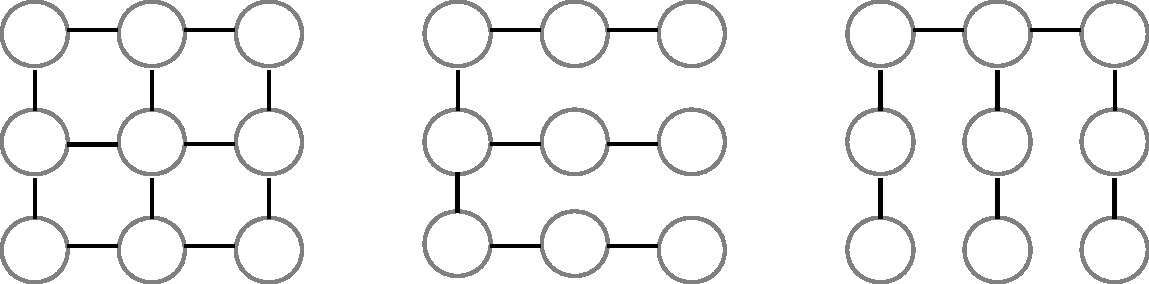
\includegraphics[width=0.8\linewidth]{img/0521.pdf} \\
	\caption{\textbf{Left}: the original grid graph. \textbf{Middle and Right}: A spanning tree decomposition with two spanning trees. Note that, in a valid decomposition, each clique will be covered by some spanning trees.}
\label{fig:trees}
\end{figure}

\begin{theorem}
	Given a set of spanning trees $\mT$ of the graph $G$, the linear programming relaxation in Eq.~(\ref{eq:lpr}) can be formulated as an equivalent convex optimization
\begin{equation}
\begin{aligned}
	&\min_{\mom} && \sum_{T \in \mT} \max_{\mnu_T \in \mM_T} \la \mom_T, \mnu_T \ra \\
	&\textrm{s.t.} && \sum_{T \in \mT} \mom_T = \mth \quad \forall T \in \mT
	%&&& \sum_{T^\prime \in \mT} \mnu_{T^\prime} = \mnu_T \quad \forall T \in \mT
\end{aligned}
\label{eq:lprdd}
\end{equation}
Here, $\mom_T$ and $\mnu_T$ can be interpreted as potentials and beliefs of the spanning tree $T$. They are of the same length as $\mth$ with zeros filled to corresponding elements where edges are not present in $G$. 
\end{theorem}
\begin{proof}
	Given a set of spanning trees $\mT$, we can construct a potential $\mth_T$ for each spanning tree $T$, such that $\sum_{\cinT} \mth_{Tc} = \mth_c$, for all $c \in C$. Then the original optimization in Eq.~(\ref{eq:lpr}) is equivalent to 
\begin{equation}
\begin{aligned}
	&\max_{\mmu \in \mM_G} && \sum_c \la \sum_{\cinT} \mth_{Tc}, \mmu_{c} \ra 
\end{aligned}
\end{equation}
By introducing a copy of $\mmu_{c}$ in each spanning tree which has the clique $c$, and constrain them to be the same as $\mmu_c$, we decompose the original problem into subproblems in spanning trees:
\begin{equation}
\begin{aligned}
	&\max_{\mmu \in \mM_G} \max_{\mnu} && \sum_c \sum_{\cinT} \la \mth_{Tc}, \mnu_{Tc} \ra \\
	&\textrm{s.t.} && \mnu_{Tc} = \mmu_c, \quad \forall T,c \\
	&&& \mnu_T \in \mM_T, \quad \forall T \in \mT
\end{aligned}
\end{equation}
where $\mnu = \{\mnu_T\}_{T \in \mT}$. \cite{Domke11} shows that the above decomposition is equivalent to 
\begin{equation}
\begin{aligned}
	&\max_{\mnu} && \sum_c \sum_{\cinT} \la \mth_{Tc}, \mnu_{Tc} \ra \\
	&\textrm{s.t.} && \mnu_{Tc} = \frac{1}{N_c} \sum_{\cinTp} \mnu_{T^\prime c}, \quad \forall T,c \\
	&&& \mnu_T \in \mM_T, \quad \forall T \in \mT
\end{aligned}
\end{equation}
where $N_c = | T \colon c \in T |$, \ie, the number of spanning trees that contain the clique $c$. 

The Lagrangian is given by
\begin{align}
	L(\mnu, \boldsymbol \lambda) = \sum_c \sum_{\cinT} \la \mth_{Tc}, \mnu_{Tc} \ra + \sum_c \sum_{\cinT} \lambda_{Tc} \bigg{(}  \mnu_{Tc} - \frac{1}{N_c} \sum_{\cinTp} \mnu_{T^\prime c} \bigg{)}
	\label{eq:lag}
\end{align}
and the dual problem is 
\begin{equation}
\begin{aligned}
	&\min_{\boldsymbol \lambda} \max_{\mnu} && L(\mnu, \boldsymbol \lambda) \\
	&\textrm{s.t.} && \mnu_T \in \mM_T, \quad \forall T \in \mT
\end{aligned}
\end{equation}
Now define $\mom_{Tc} = \mth_{Tc} + \lambda_{Tc} - \frac{1}{N_c} \sum_{\cinTp} \lambda_{T^\prime c}$. Observing that
\begin{align}
	\sum_{\cinT} \mom_{Tc} = \sum_{\cinT} \mth_{Tc} + \lambda_{Tc} - \frac{1}{N_c} \sum_{\cinTp} \lambda_{T^\prime c} = \sum_{\cinT} \mth_{Tc} = \mth_c
\end{align}
thus we can transfer Lagrangian multipliers $\lambda_{Tc}$ into $\mom_{Tc}$, by substituting $\mth_{Tc} = \mom_{Tc} - \lambda_{Tc} + \frac{1}{N_c} \sum_{\cinTp} \lambda_{T^\prime c}$ into Eq.~\ref{eq:lag}. The dual problem can be rewriten accordingly as 
\begin{equation}
\begin{aligned}
	&\min_{\mom} \max_{\mnu} && \sum_c \sum_{\cinT} \la \mom_{Tc}, \mnu_{Tc} \ra \\
	&\textrm{s.t.} && \sum_{\cinT} \mom_{Tc} = \mth_c, \quad \forall c \\
	&&& \mnu_T \in \mM_T, \quad \forall T \in \mT
\end{aligned}
\end{equation}
which can be simplified as the same form as Eq.~\ref{eq:lprdd}.
\end{proof}

Note that Eq.~(\ref{eq:lprdd}) is a constrained convex optimization and consists of subproblems with respect to each tree of the form 
\begin{align}
	S(\mom_T) = \max_{\mnu_T} \la \mom_T, \mnu_T \ra,
\end{align}
which can be solved exactly by running the sum-product message passing on the tree $T$ \cite{Yanover06}.

\section{Algorithm}
%Describe the algorithm in details and discuss the advantages and disadvantages (if any) of the algorithm for the problem in consideration.

Let $M(\mom) = \sum_{T \in \mT} S(\mom_T)$ denote the master problem of Eq.~(\ref{eq:lprdd}). We will use the Frank-Wolfe algorithm \cite{JaggiICML13} to solve this constraint convex optimization. Briefly, the algorithm iterates the following steps:

\begin{algorithm}
\caption{Frank-Wolfe Algorithm}
\label{frankwolfe}
\begin{algorithmic}
\Require{Initialize: $\mom^k = $ initial potentials}
\Repeat
	\State{Direction: $\ms \leftarrow \argmin_{\mom} \la \mom, \nabla M(\mom^k) \ra$}
	\State{\indent $\textrm{subject to } \sum_{T \in \mT} \mom_T = \mth$.}
	\State{Step size: $\gamma \leftarrow \frac{2}{2-k}$}
	\State{Update: $\mom^{k+1} \leftarrow \mom^k + \gamma (\ms - \mom^k)$.}
\Until{$| M(\mom^k) - M(s) | < \epsilon$}
\end{algorithmic}
\end{algorithm}

Since $\frac{\partial M(\mom)}{\partial \mom_T } = \frac{\partial S(\mom)}{\partial \mom_T } = \mnu_T^*$, by Danskin's theorem, the direction step is trivial, which involves solving a linear programming with a single linear constraint. Then the step size $\gamma$ is updated so that it becomes smaller with each iteration. Finally, $\mom$ is updated where the descent direction is computed based on the computed direction and step size. This is repeated for $K$ iterations or when the duality gap is sufficiently small: $| M(\mom^k) - M(s) | < \epsilon$.

\subsection{Convergence Analysis}

Here we present the convergence analysis of the Frank-Wolfe algorithm. TODO

\section{Experiments}


%Provide simulation results and discuss the results.

%\subsection{Subsection Heading Here}
%Subsection text here.

% command of the stfloats package.

We evaluate our approach on computer vision tasks that transform a structured input to a structured output. These computer vision tasks employ the conditional random field where the structured output consists of labels for every pixel and the structured input are image features. CRF inference is addressed with our approach.

We evaluate our approach on two tasks: image denoising and scene labeling. The image denoising task involves a toy dataset, which provides a good check that our approach is working. We then evaluate our approach on the scene labeling task. We evaluate scene labeling on the Stanford Background dataset, a standard dataset of natural scenes used in computer vision.

\subsection{Image Denoising}

Our first task is to evaluate our approach for image denoising. Given a corrupted, noisy image, the task of inference is to recover the original image; in other words, we want to denoise the image. Fig. \ref{fig:denoisingdemo} demonstrates the denoising task.

\begin{figure}
\centering
\includegraphics[width=0.33\columnwidth]{img/originalX.png}\hfill%
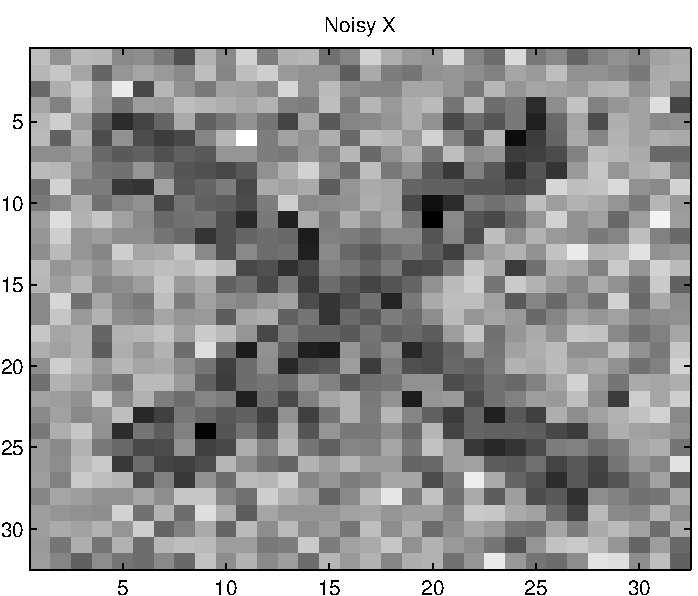
\includegraphics[width=0.33\columnwidth]{img/noisyX.png}\hfill%
\includegraphics[width=0.33\columnwidth]{img/inferX.png}
\caption{Illustration of the image denoising task. The {\bf left} figure is the original (ground truth) image. The {\bf middle} figure is the corrupted image. The {\bf right} figure is a result of our inference task using the baseline ICM approach. The original image is reconstructed from the noise.}
\label{fig:denoisingdemo}
\end{figure}

{\bf Setup.} We model the CRF as a regular grid of pixels (i.e. every node corresponds to a pixel) with 4-connected neighbors. The unary potentials consist of pixel intensities and pairwise potentials employ the Pott's model to encourage smoothness. This graphical model is decomposed into two spanning tree graphical models that is used for dual decomposition as in Fig. \ref{fig:trees}.

{\bf Dataset.} Our dataset consists of 20 binary images with various white circles placed at different locations over a black background. The dataset is corrupted with Gaussian noise (i.e. every pixel in the image is changed by a value sampled from a Gaussian distribution) for input into the denoising task. This noisy image is a grayscale image.

{\bf Metrics.} Our metric is pixel accuracy. Every pixel of the inferred image is compared to the groundtruth image.

{\bf Baselines.} The baseline inference algorithm is Iterated Conditioned Modes (ICM). Empirically this yields the best result among other possible baseline inference algorithms. TODO

{\bf Quantitative Results.} We present some quantitative results in Table \ref{tab:denoising_accuracy}. TODO

\begin{table}[!h]
    \centering
	    \begin{tabular}{|c|c|}
	    	\hline
			Approach & Pixel Accuracy \\ \hline
			Baseline & 98.37\% \\ \hline
			Ours & --- \\ \hline
		\end{tabular}\\
    \caption{Pixel accuracy on the image denoising task comparing our approach and the baseline approach. Pixel accuracy is the percentage of correct labels over all pixels. TODO}\label{tab:denoising_accuracy}
\end{table}

{\bf Duality Gap.} We demonstrate that the duality gap decreases as the number of iterations increases in Fig. \ref{fig:denoisinggap}. TODO

\begin{figure}
\centering
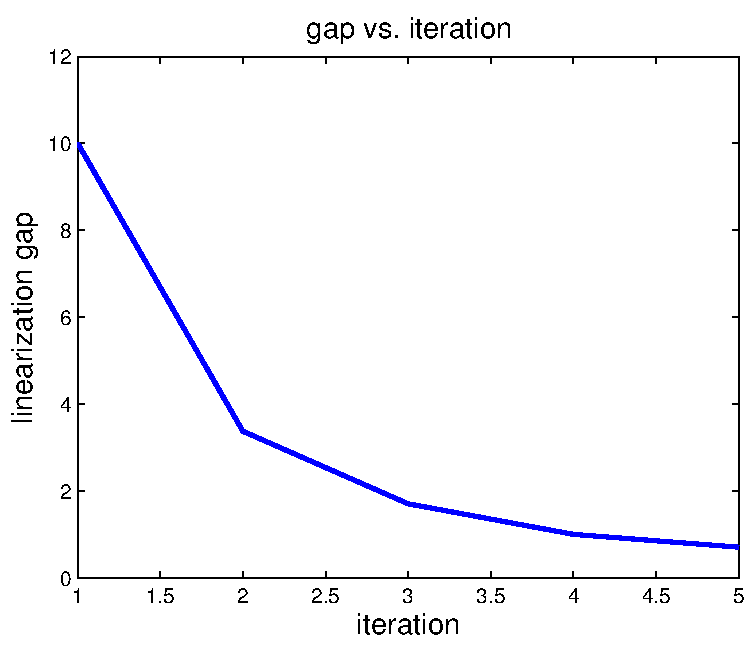
\includegraphics[width=.75\columnwidth]{img/fwdd_gap.pdf}
\caption{The duality gap decreases as the number of iterations increases.}
\label{fig:denoisinggap}
\end{figure}

{\bf Qualitative Results.} We present some qualitative results for image denoising in Fig. \ref{fig:denoisingresults}. We note that our approach yields good results. The baseline approach is performing slightly better than our approach. TODO

\begin{figure}
\centering
\begin{minipage}{1\columnwidth}
	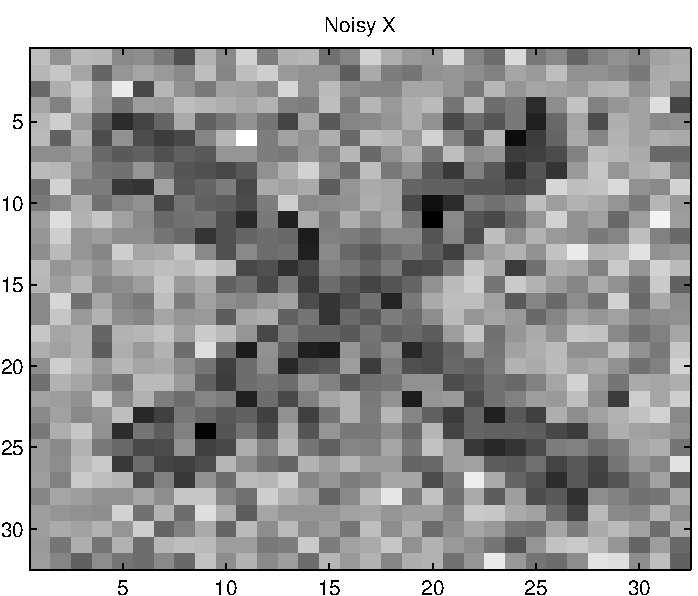
\includegraphics[width=0.33\columnwidth]{img/noisyX.png}\hfill%
	\includegraphics[width=0.33\columnwidth]{img/inferX.png}\hfill%
	\includegraphics[width=0.33\columnwidth]{img/inferX.png}
\end{minipage}
\begin{minipage}{1\columnwidth}
	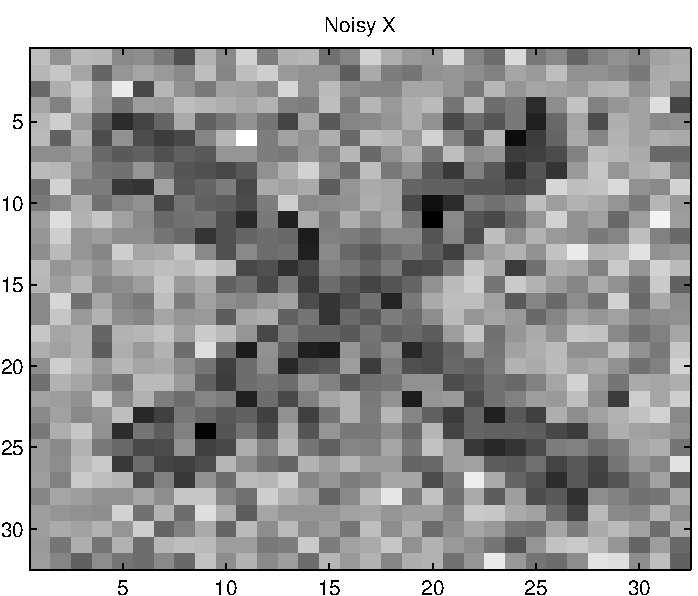
\includegraphics[width=0.33\columnwidth]{img/noisyX.png}\hfill%
	\includegraphics[width=0.33\columnwidth]{img/inferX.png}\hfill%
	\includegraphics[width=0.33\columnwidth]{img/inferX.png}
\end{minipage}
\begin{minipage}{1\columnwidth}
	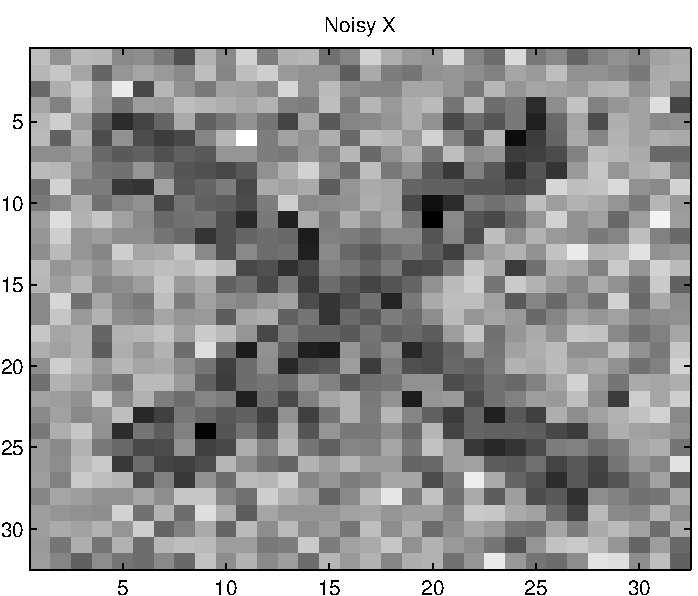
\includegraphics[width=0.33\columnwidth]{img/noisyX.png}\hfill%
	\includegraphics[width=0.33\columnwidth]{img/inferX.png}\hfill%
	\includegraphics[width=0.33\columnwidth]{img/inferX.png}
\end{minipage}
\caption{Image denoising results. The {\bf left} column contains some corrupted images. The {\bf middle} column are the results of inference using the baseline ICM approach. The {\bf right} column are the results of inference using our approach.}
\label{fig:denoisingresults}
\end{figure}

We also demonstrate the effect of dual decomposition in \ref{fig:denoisingdecomposition}. We see that the marginal beliefs for the tree decompositions make sense based on the ``smearing'' artifacts. Each tree decomposition consists of pairwise potentials that are only present in the vertical or horizontal direction. The results of tree decomposition 1 shows ``smearing'' in the horizontal direction, which aligns with the spanning tree model with horizontal pairwise potentials. We also see that the final marginal beliefs ``average out'' these artifacts to yield a good solution.

\begin{figure}
\centering
\begin{minipage}{1\columnwidth}
	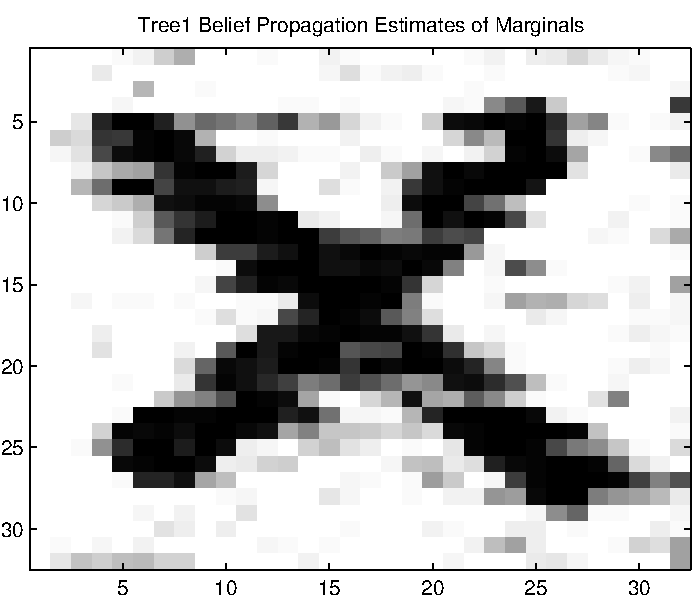
\includegraphics[width=0.5\columnwidth]{img/tree1_bel.pdf}\hfill%
	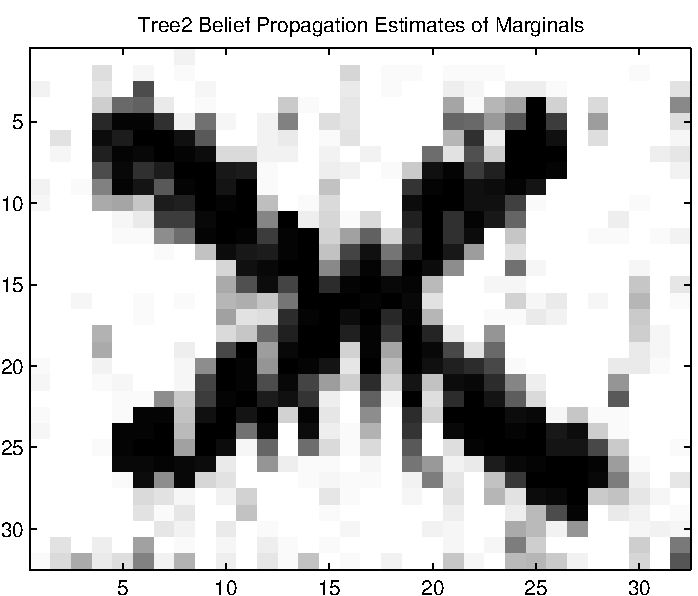
\includegraphics[width=0.5\columnwidth]{img/tree2_bel.pdf}
\end{minipage}
\begin{minipage}{1\columnwidth}
	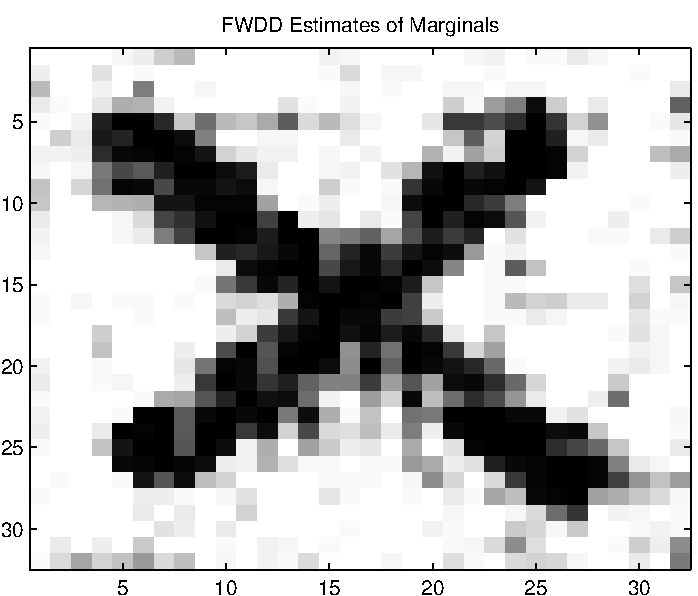
\includegraphics[width=0.5\columnwidth]{img/fwdd_bel.pdf}\hfill%
	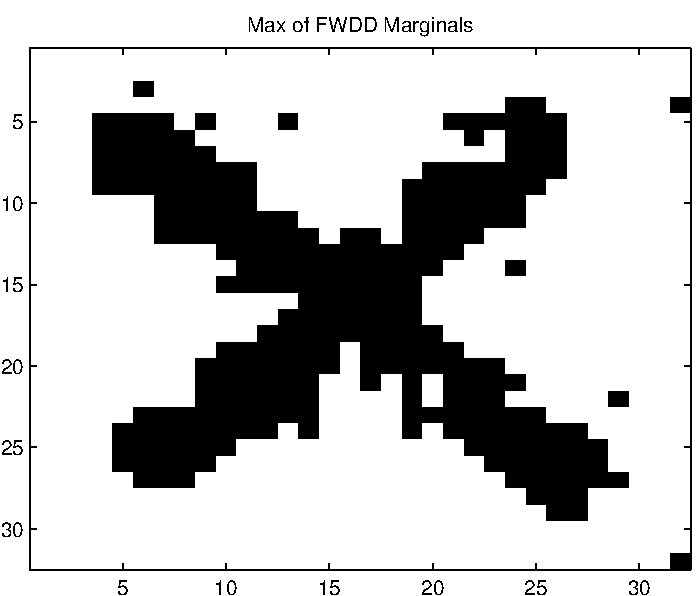
\includegraphics[width=0.5\columnwidth]{img/fwdd_max_bel.pdf}
\end{minipage}
\caption{The {\bf top left} figure shows the marginal beliefs of tree decomposition 1 and the {\bf top right} figure shows the marginal beliefs of tree decomposition 2. The {\bf bottom left} figure fuses the results of the two decompositions into the final marginal beliefs. The {\bf bottom right} figure gives the final denoised image from the final marginal beliefs.}
\label{fig:denoisingdecomposition}
\end{figure}


\subsection{Scene Labeling}

We consider the task of scene labeling on a standard computer vision dataset for general images of natural scenes, the Stanford Background Dataset. We formulate the scene labeling problem as an optimization problem and use our proposed algorithm for performing inference. The task of scene labeling is to label every pixel in an image with a semantic class.

{\bf Setup.} The image structure can be modeled with a CRF where the structured output consists of a semantic label for every pixel and the structured input are image features. The unary potentials for each pixel corresponds to the features around a neighborhood of that pixel. The features are color and texture. The pairwise potentials for every pair of neighboring pixels models the compatibility of the neighbor label assignments, which is used for smoothness. Similar to the image denoising task, this graphical model is also decomposed into two spanning tree graphical models that is used for dual decomposition as in Fig. \ref{fig:trees}.

{\bf Dataset.} Our dataset is the Stanford Background Dataset. This is a standard dataset consisting of 715 general images of natural scenes and 8 semantic classes.

{\bf Metrics.} Similar to the image denoising task, we evaluate with pixel accuracy.

{\bf Baselines.} The baseline approaches include ---. TODO

{\bf Quantitative Results.} We present some quantitative results in Table \ref{tab:res-sb}. TODO

\begin{table}[ht]
\caption{The comparison of average pixel-wise accuracy on the Stanford
  background dataset. \textbf{Left}: State-of-the-art
  results. \textbf{Right}: Our results. TODO \label{tab:res-sb}}
%Note that for RT, all methods use the RNN features, whose dimension
%is empirically set to 50, which is the number of hidden units. For
%BST, all methods use the raw features, whose dimension is 140 as
%aforementioned.}
\centering
\begin{minipage}[b]{0.65\linewidth}
\centering
\scalebox{0.9}{
\begin{tabular}{|l|r|}
\hline
\hline
%\multicolumn{3}{|c|}{RNN Trees}\\
%\hline
\multicolumn{1}{|c}{Methods} & \multicolumn{1}{|c|}{Acc.} \\
\hline
%Pixel CRF \cite{Gould_ICCV09}            					& 74.3 \\
Region Energy \cite{Gould_ICCV09}            				& 76.4 \\
SHL \cite{munoz-bagnell-hebert-10} 							& 76.9 \\
RNN \cite{socher-lin-ng-manning-11}            				& 78.1 \\
ConvNet \cite{LeCun_PAMI13}									& 78.8 \\
ConvNet + NN \cite{LeCun_PAMI13}							& 80.4 \\
ConvNet + CRF \cite{LeCun_PAMI13}							& 81.4 \\
Pylon (No Bnd) \cite{lempitsky-vedaldi-zisserman-11}		& 81.29 \\
Pylon \cite{lempitsky-vedaldi-zisserman-11}					& 81.90 \\
\hline
\hline
\end{tabular}
}
\end{minipage}\hfill
\begin{minipage}[b]{0.35\linewidth}
\centering
\scalebox{0.9}{
\begin{tabular}{|l|l|r|}
\hline
\hline
%\multicolumn{3}{|c|}{Berkeley Seg. Trees} \\
%\hline
\multicolumn{2}{|c|}{Methods} & \multicolumn{1}{|c|}{Acc.} \\
\hline
\multirow{4}{*}{RT}  %& LR (RNNfeat)								& 78.90 & 88.13\\
					 & LR								& 79.04 \\%& 88.14\\
					 & CRF								& 77.63 \\
					 & Tree-Cut							& 81.06 \\%& 89.16\\
					 & Upper Bound						& 93.28 \\%& 97.58\\
\hline
\multirow{4}{*}{BST} & LR								& 76.33 \\%& 84.43\\
 & CRF													& 76.81 \\
 & Tree-Cut												& 77.16 \\%& 84.30\\
 & Upper Bound											& 95.78 \\%& 97.20\\
\hline
\hline
\end{tabular}
}
\end{minipage}
\end{table}

{\bf Qualitative Results.} We present some qualitative results in Fig. \ref{fig:scenelabelingresults}. TODO

\begin{figure}
\centering
\begin{minipage}{1\columnwidth}
	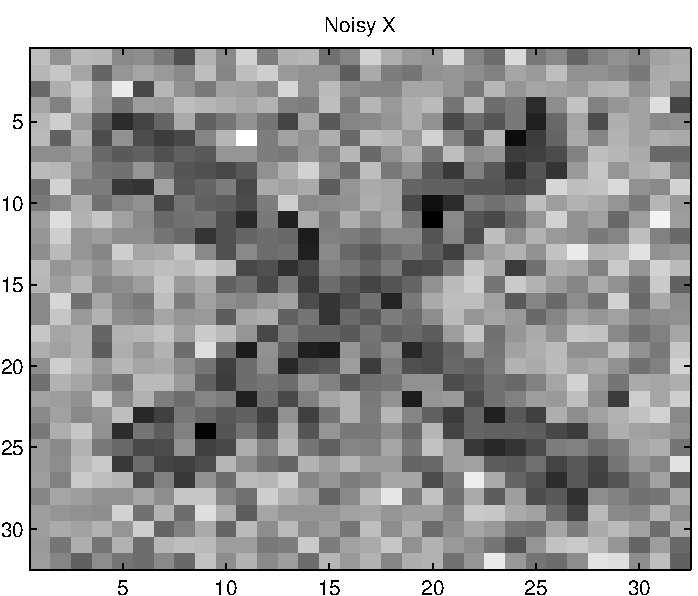
\includegraphics[width=0.33\columnwidth]{img/noisyX.png}\hfill%
	\includegraphics[width=0.33\columnwidth]{img/inferX.png}\hfill%
	\includegraphics[width=0.33\columnwidth]{img/inferX.png}
\end{minipage}
\begin{minipage}{1\columnwidth}
	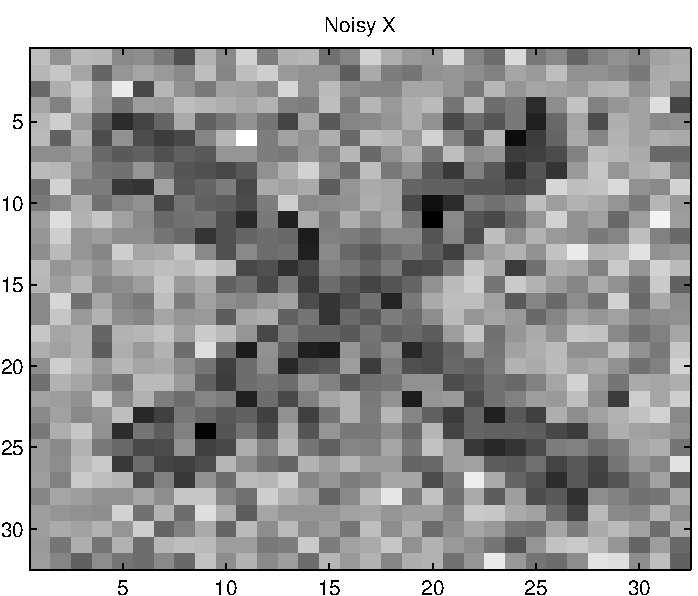
\includegraphics[width=0.33\columnwidth]{img/noisyX.png}\hfill%
	\includegraphics[width=0.33\columnwidth]{img/inferX.png}\hfill%
	\includegraphics[width=0.33\columnwidth]{img/inferX.png}
\end{minipage}
\begin{minipage}{1\columnwidth}
	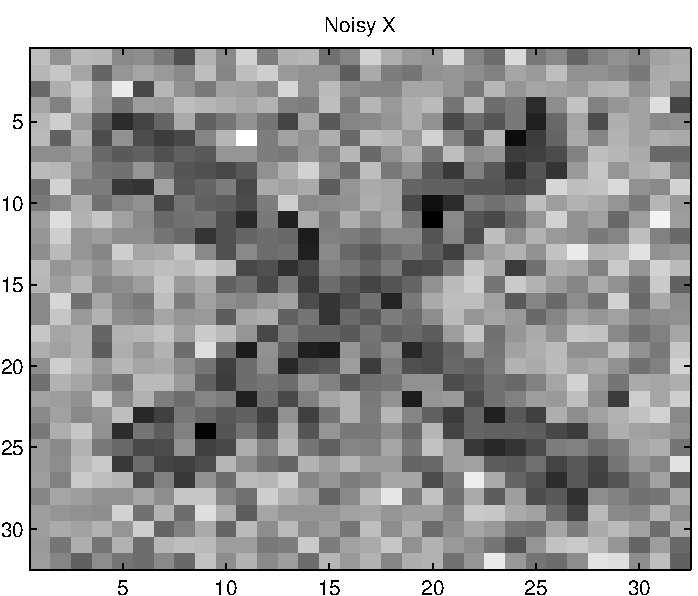
\includegraphics[width=0.33\columnwidth]{img/noisyX.png}\hfill%
	\includegraphics[width=0.33\columnwidth]{img/inferX.png}\hfill%
	\includegraphics[width=0.33\columnwidth]{img/inferX.png}
\end{minipage}
\caption{Scene labeling results. The {\bf left} column contains the groundtruth images. The {\bf middle} column are the results of inference using a baseline approach. The {\bf right} column are the results of inference using our approach. TODO}
\label{fig:scenelabelingresults}
\end{figure}

\section{Conclusion}
%The conclusion goes here.

We have presented an approach for solving the MAP inference problem for CRFs. Our formulation of the dual problem to MAP inference allows for efficient inference by solving subproblems. The Frank-Wolfe algorithm is able to solve our constrained convex optimization formulation. We evaluated our approach on image denoising and scene labeling and show that we are getting good results. Our formulation and algorithm is a promising framework for MAP inference of CRFs.

% conference papers do not normally have an appendix

% use section* for acknowledgement
\section*{Contributions of Individual Team members}

Hu primarily contributed to the theory and formulations while Lam primarily contributed to the codebase, although both Hu and Lam contributed across the whole project. Recognition is given to Hu for coming up with the project idea.

% trigger a \newpage just before the given reference
% number - used to balance the columns on the last page
% adjust value as needed - may need to be readjusted if
% the document is modified later
%\IEEEtriggeratref{8}
% The "triggered" command can be cIterated Conditioned Modes (ICM). Empirically this yields the best result among other possible baseline inference algorithms.hanged if desired:
%\IEEEtriggercmd{\enlargethispage{-5in}}

% references section

% can use a bibliography generated by BibTeX as a .bbl file
% BibTeX documentation can be easily obtained at:
% http://www.ctan.org/tex-archive/biblio/bibtex/contrib/doc/
% The IEEEtran BibTeX style support page is at:
% http://www.michaelshell.org/tex/ieeetran/bibtex/
\bibliographystyle{IEEEtran}
% argument is your BibTeX string definitions and bibliography database(s)
\bibliography{proj}
%
% <OR> manually copy in the resultant .bbl file
% set second argument of \begin to the number of references
% (used to reserve space for the reference number labels box)
%\begin{thebibliography}{1}
%
%\bibitem{IEEEhowto:kopka}
%H.~Kopka and P.~W. Daly, \emph{A Guide to \LaTeX}, 3rd~ed.\hskip 1em plus
%  0.5em minus 0.4em\relax Harlow, England: Addison-Wesley, 1999.
%
%\end{thebibliography}



% that's all folks
\end{document}


